\chapter{Design}
The web application needs to handle a big amount of data, so we decided to use a combination of different databases to store and manage the data. We will use a document database to store users, media contents and reviews data, and a graph database to store relationships between users and media content. This will allow us to efficiently store and retrieve data, as well as handle complex relationships between data. 

\section{Document Database}
For the document database, we will use MongoDB. MongoDB is a NoSQL database that stores data in flexible, JSON-like documents. It is a popular choice for applications that require flexibility and scalability. MongoDB is a document database, which means it stores data in JSON-like documents. These documents are flexible, meaning they can have different fields and structures. This makes MongoDB a good choice for applications that require flexibility in their data model. MongoDB is also a scalable database, meaning it can handle large amounts of data and traffic. It is designed to scale out, meaning you can add more servers to handle more traffic. This makes MongoDB a good choice for applications that need to scale quickly.
\newline
\newline
\textbf{Collections}
The database will have the following collections:
\begin{itemize}
    \item Anime: This collection will store information about anime, such as titles, tags, and synopsis.
    \item Manga: This collection will store information about manga, such as titles, genres, and authors.
    \item Reviews: This collection will store user ratings and comments for media content.
    \item Users: This collection will store user data, such as usernames, passwords, email addresses, gender and location.

\end{itemize}
\newpage
\textbf{MongoDB document example}
\newline
Anime:
\begin{mdframed}[backgroundcolor=yellow!20, innerleftmargin=10pt, innerrightmargin=10pt]
    \begin{lstlisting}[language=java]
{
  "_id": "65789bb52f5d29465d0abcfb",
  "title": "0",
  "type": "SPECIAL",
  "episodes": 1,
  "status": "FINISHED",
  "picture": "https://cdn.myanimelist.net/images/anime/12/81160.jpg",
  "tags": [
    "drama",
    "female protagonist",
    "indefinite",
    "music",
    "present"
  ],
  "producers": "Sony Music Entertainment",
  "studios": "Minakata Laboratory",
  "synopsis": "This music video tells how a shy girl with a secret love and curiosity...",
  "latest_reviews": [
    {
      "id": "657b301306c134f18884924c",
      "date": "2023-10-03T22:00:00.000+00:00",
      "rating": 4,
      "user": {
        "id": "6577877ce68376234760745c",
        "username": "Tolstij_Trofim",
        "picture": "https://thypix.com/wp-content/uploads/2021/10/manga-profile-picture-10..."
      }
    },
  ],
  "anime_season": {
    "season": "FALL",
    "year": 2013
  },
  "average_rating": 6.7,
  "avg_rating_last_update": true,
  "likes": 4
}
    \end{lstlisting}
\end{mdframed}

\newpage
Manga:
\begin{mdframed}[backgroundcolor=yellow!20, innerleftmargin=10pt, innerrightmargin=10pt]
    \begin{lstlisting}[language=java]
{
  "_id": "657ac61bb34f5514b91ea223",
  "title": "Berserk",
  "type": "MANGA",
  "status": "ONGOING",
  "genres": [
    "Action",
    "Adventure",
    "Award Winning",
    "Drama",
    "Fantasy",
    "Horror",
    "Supernatural"
  ],
  "themes": [
    "Gore",
    "Military",
    "Mythology",
    "Psychological"
  ],
  "demographics": [
    "SEINEN"
  ],
  "authors": [
    {
      "id": 1868,
      "role": "Story & Art",
      "name": "Kentarou Miura"
    },
    {
      "serializations": "Young Animal"
    }
  ],
  "synopsis": "Guts, a former mercenary now known as the \"Black Swordsman,\" is out fo...",
  "title_english": "Berserk",
  "start_date": "1989-08-25T00:00:00.000+00:00",
  "picture": "https://cdn.myanimelist.net/images/manga/1/157897l.jpg",
  "average_rating": 3.33,
  "latest_reviews": [
    {
      "user": {
        "id": "6577877be683762347605ce7",
        "username": "calamity_razes",
        "picture": "https://imgbox.com/7MaTkBQR"
      },
      "date": "2012-12-15T00:00:00.000+00:00",
      "comment": "An insult to the art of manga; avoid at all costs.",
      "id": "657b302206c134f18886f5ef"
    },
  ],
  "anime_season": {
    "season": "FALL",
    "year": 2013
  },
  "average_rating": 6.7,
  "avg_rating_last_update": true,
  "likes": 4
}
    \end{lstlisting}
\end{mdframed}

\newpage
Reviews:
\begin{mdframed}[backgroundcolor=yellow!20, innerleftmargin=10pt, innerrightmargin=10pt]
    \begin{lstlisting}[language=java]
{
  "_id": "657b300806c134f18882f2f1",
  "user": {
    "id": "6577877be68376234760596d",
    "username": "Dragon_Empress",
    "picture": "images/account-icon.png",
    "location": "Columbus, Georgia",
    "birthday": "1987-07-29T00:00:00.000+00:00",
    "rating": 7
  },
  "anime": {
    "id": "65789bbc2f5d29465d0b18b7",
    "title": "Slayers Revolution",
    "date": "2023-07-23T06:27:54.000+00:00",
    "comment": "Above-average quality in animation and soundtrack."
  }
}
    \end{lstlisting}
\end{mdframed}

Users:
\begin{mdframed}[backgroundcolor=yellow!20, innerleftmargin=10pt, innerrightmargin=10pt]
    \begin{lstlisting}[language=java]
{
  "_id": "6577877be683762347605859",
  "email": "xdavis@example.com",
  "password": "290cb38a679d5eb68d11b9ea1e21f48234eba6de19f95612dbcb70ce0c7e4e78",
  "description": "Liberating the mind from stress with the power of anime zen.",
  "picture": "https://thypix.com/wp-content/uploads/2021/10/manga-profile-picture-44",
  "username": "Xinil",
  "gender": "Male",
  "birthday": "1985-03-04T00:00:00.000+00:00",
  "location": "Libya",
  "joined_on": "2014-05-29T00:00:00.000+00:00",
  "app_rating": 5,
  "followed": 40,
  "followers": 29
}
    \end{lstlisting}
\end{mdframed}


The field \texttt{"app\_rating"} is used to know the general satisfaction of the user with the application.


\subsection{Indexes}

We created two indexes in the reviews collection to improve query performance. One for the users id and another for the anime and manga id. This will allow us to quickly retrieve reviews for a specific user or media content. 


\newpage
\section {MongoDB queries}
Some of the most important MongoDB queries for analytic and suggestion porpouses. 


\textbf{USERS:}
\begin{itemize}
  \item GetDistribution query to get the user's location, gender, birthday year that gave the highest rating to the application:
  
\end{itemize}
\begin{lstlisting}[language=JavaScript, caption=GetDistribution]
  // Match stage to filter documents where 'criteriaOfSearch' exists
  db.collection.aggregate([
      {
          $match: {
              [criteriaOfSearch]: { $exists: true }
          }
      },
      // Project stage to include 'criteriaOfSearch' and 'app_rating' fields
      {
          $project: {
              [criteriaOfSearch]: 1,
              app_rating: 1
          }
      },
      // Group stage to count occurrences of each 'criteriaOfSearch'
      {
          $group: {
              _id: "$" + criteriaOfSearch,
              count: { $sum: 1 }
          }
      },
      // Sort stage to sort documents by 'count' in descending order
      {
          $sort: {
              count: -1
          }
      }
  ]);
  \end{lstlisting}
  


\textbf{ANIME/MANGA:}

\begin{itemize}

\item GetBestCriteria query, the criteria can be genres, demographics, themes, authors and serialization for manga; tags, producers, studios for anime:
\begin{lstlisting}[language=JavaScript, caption=GetBestCriteria]
  db.collection.aggregate([
      // Match stage to filter documents where 'criteria' exists and 'average_rating' is not null
      {
          $match: {
              criteria: { $exists: true },
              average_rating: { $ne: null }
          }
      },
      // Unwind stage to deconstruct the 'criteria' array field
      {
          $unwind: "$" + criteria
      },
      // Group stage to calculate the average rating for each criteria
      {
          $group: {
              _id: "$" + criteria,
              criteria_average_rating: { $avg: "$average_rating" }
          }
      },
      // Sort stage to sort documents by 'criteria_average_rating' in descending order
      {
          $sort: {
              criteria_average_rating: -1
          }
      },
      // Skip stage to skip the first 'pageOffset' documents
      {
          $skip: pageOffset
      },
      // Limit stage to limit the results to 25 documents
      {
          $limit: 25
      }
  ]);
  \end{lstlisting}

\end{itemize}

\textbf{REVIEWS:}

\begin{itemize}
\item GetMediaContentRatingByYear query to get the average rating of media content by year:
\end{itemize}


\begin{lstlisting}[language=JavaScript, caption=GetMediaContentRatingByYear]
  // Match stage to filter documents based on specified conditions
  db.collection.aggregate([
      {
          $match: {
              [`${nodeType}.id`]: new ObjectId(mediaContentId),
              rating: { $exists: true },
              date: { $gte: startDate, $lt: endDate }
          }
      },
      // Group stage to group documents by year and calculate the average rating
      {
          $group: {
              _id: { $year: "$date" },
              average_rating: { $avg: "$rating" }
          }
      },
      // Project stage to shape the output documents
      {
          $project: {
              _id: 0,
              year: "$_id",
              average_rating: 1
          }
      },
      // Sort stage to sort documents by year in ascending order
      {
          $sort: { year: 1 }
      }
  ]);
  \end{lstlisting}


\begin{itemize}
  \item SuggestMediaContent query to suggest media content based on common criteria, like birthday or location:
  
\end{itemize}

\begin{lstlisting}[language=JavaScript, caption=SuggestMediaContent]
  db.collection.aggregate([
  {
    // Match documents based on a dynamic user criteria
    $match: {
      ["user." + criteriaType]: criteriaValue
    }
  },
  {
    // Group documents by node type ID and calculate the first title and average rating
    $group: {
      _id: "$" + nodeType + ".id", // Group by the node type's ID
      title: { $first: "$" + nodeType + ".title" }, // Get the first title in the group
      average_rating: { $avg: "$rating" } // Calculate the average rating for the group
    }
  },
  {
    // Sort the grouped documents by average rating in descending order
    $sort: { average_rating: -1 }
  },
  {
    // Limit the number of results to the page size constant
    $limit: Constants.PAGE_SIZE
  }
]);
\end{lstlisting}







\subsection {CRUD operations}
\begin{itemize}
    \item Create: This operation will allow users to create new documents in the database. For example, users can create new reviews for anime and manga.
    \item Read: This operation will allow users to read documents from the database. For example, users can read information about anime and manga and about other users.
    \item Update: This operation will allow users to update documents in the database. For example, users can update their reviews for anime and manga, they can also update their own profile, the manager can update media contents.
    \item Delete: This operation will allow users to delete documents from the database. For example, users can delete their reviews for anime and manga, the manager can delete media contents.
\end{itemize}

\newpage
\section{Graph Database}
For the graph database, we will use Neo4j. Neo4j is a graph database that stores data in nodes and relationships. It is a popular choice for applications that require complex relationships between data. Neo4j is a graph database, which means it stores data in nodes and relationships. Nodes represent entities, such as users or products, and relationships represent connections between nodes. This makes Neo4j a good choice for applications that require complex relationships between data. Neo4j is also a scalable database, meaning it can handle large amounts of data and traffic. It is designed to scale out, meaning you can add more servers to handle more traffic. This makes Neo4j a good choice for applications that need to scale quickly.



\textbf{Nodes}



The database will have the following nodes:
\begin{itemize}
    \item User: This node will store information about users, such as id, usernames, and picture.
    \item Anime: This node will store information about anime, such as id, titles and picture.
    \item Manga: This node will store information about manga, such as id, titles and picture.
\end{itemize}

\textbf{Relationships}


The database will have the following relationships:
\begin{itemize}
    \item LIKE: This relationship will connect users to anime and manga nodes. It will store the date when the user liked the media content.
    \item FOLLOW: This relationship will connect users to other users. 
\end{itemize}

\begin{figure}[htbp]
    \centering
    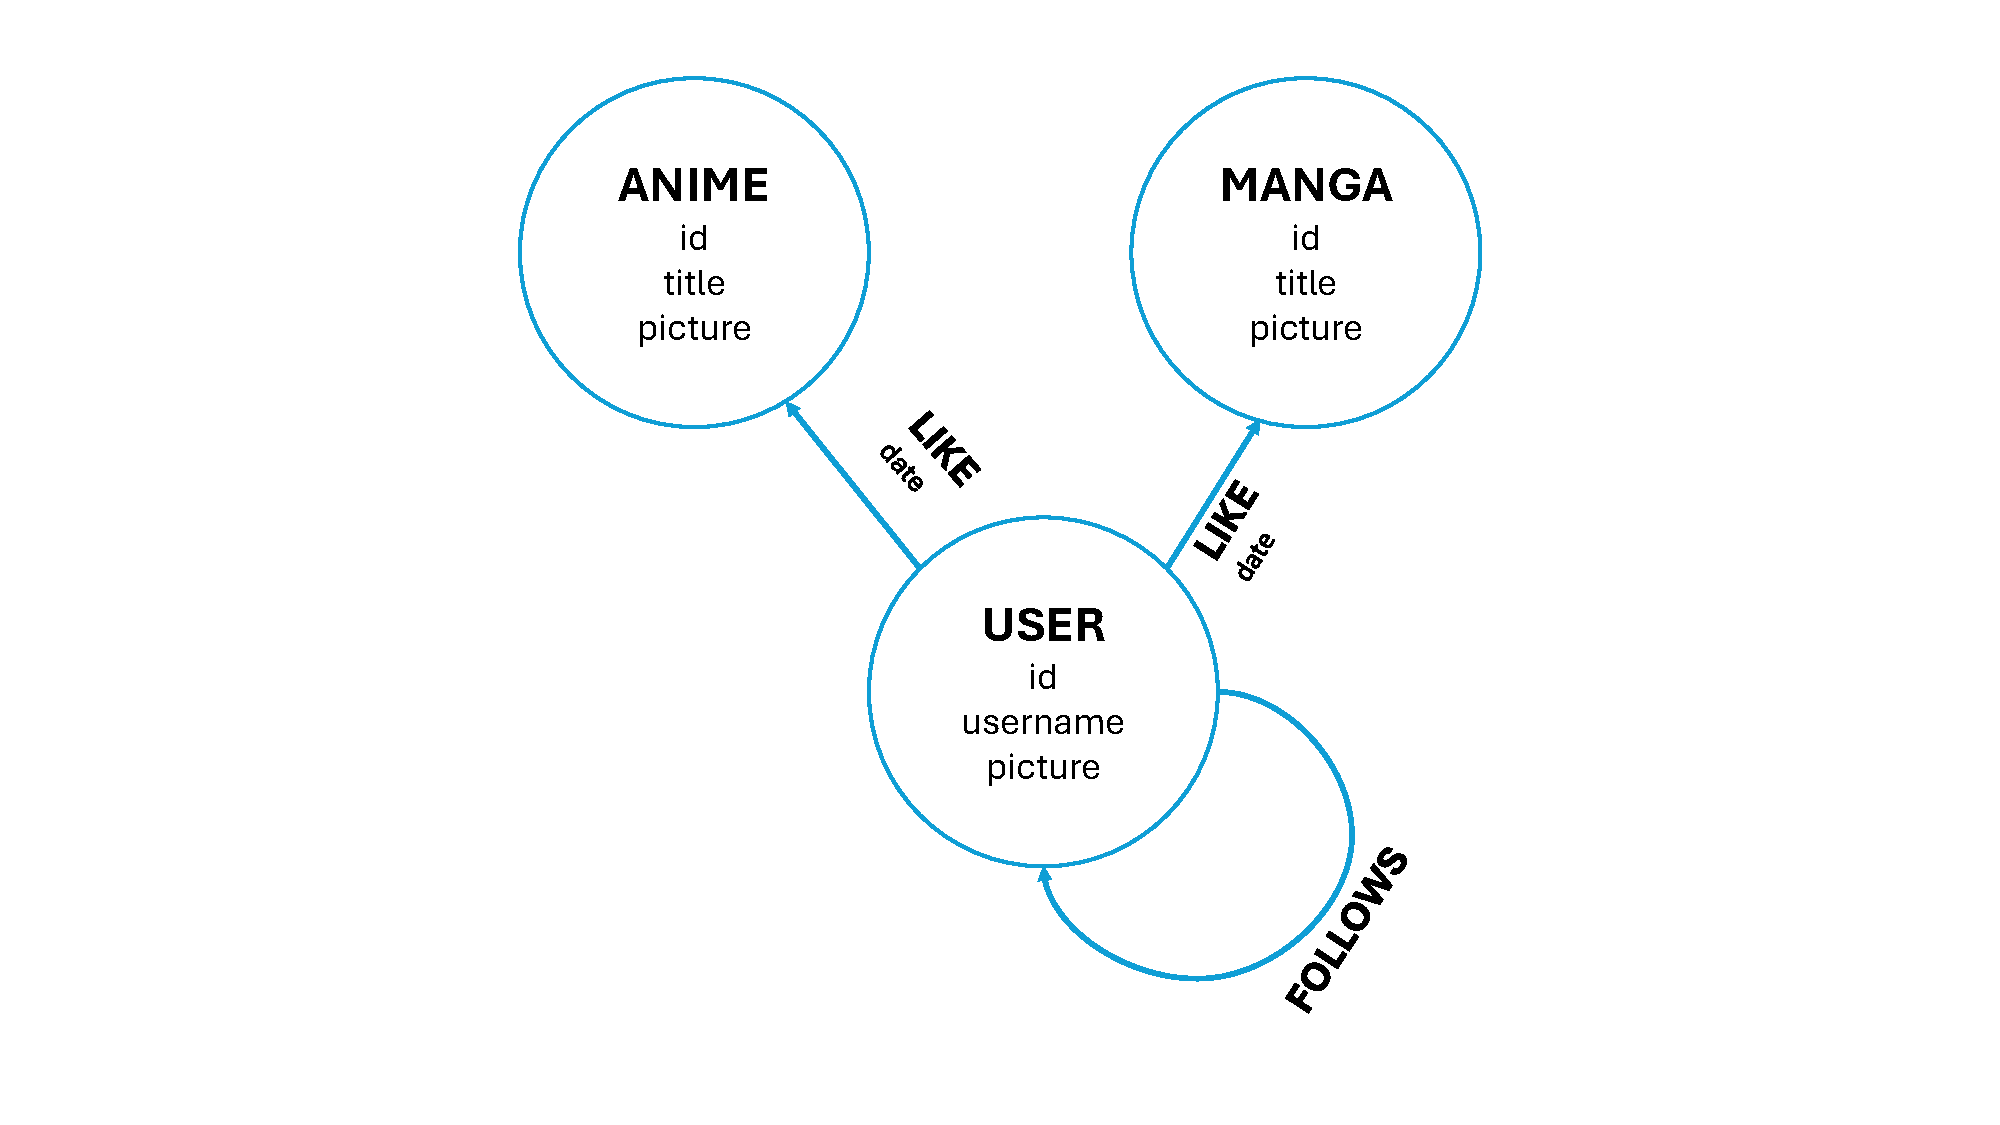
\includegraphics[width=\textwidth]{Media/graph.pdf}
    \caption{GraphDB}
    \label{fig:GraohDB}
\end{figure}

\newpage
\section{GraphDB queries}
Some of the most important Neo4j queries for analytic and suggestion porpouses.


\textbf{USERS:}

\begin{itemize}
  \item Suggest other users followings in common:
\end{itemize}
\begin{lstlisting}[language=Cypher, caption=SuggestUsersByCommonFollowings]

MATCH (u:User {id: $userId})-[:FOLLOWS]->(following:User)<-[:FOLLOWS]-(suggested:User) 
WHERE NOT (u)-[:FOLLOWS]->(suggested) AND u <> suggested 
WITH suggested, COUNT(DISTINCT following) AS commonFollowers 
WHERE commonFollowers > 5 
RETURN suggested as user, commonFollowers 
ORDER BY commonFollowers DESC 
LIMIT $n
\end{lstlisting}

\begin{itemize}
  \item Suggest other users likes in common:
\end{itemize}
\begin{lstlisting}[language=Cypher, caption=SuggestUsersByCommonLikes]
  MATCH (u:User {id: $userId})-[r:LIKE]->(media:Manga)<-[:LIKE]-(suggested:User) 
  WHERE u <> suggested AND r.date >= $date
  WITH suggested, COUNT(DISTINCT media) AS commonLikes
  WHERE commonLikes > $min
  RETURN suggested AS user, commonLikes
  ORDER BY commonLikes DESC
  LIMIT $n
\end{lstlisting}



\textbf{ANIME/MANGA:}

\begin{itemize}
  \item Suggest anime and manga based on following in common:
\end{itemize}
\begin{lstlisting}[language=Cypher, caption=GetSuggestedByFollowings]
  MATCH (u:User {id: $userId})-[:FOLLOWS]->(f:User)-[r:LIKE]->(a:Anime)
  WHERE NOT (u)-[:LIKE]->(a) AND r.date >= $startDate
  WITH a, COUNT(DISTINCT f) AS num_likes
  RETURN a AS anime
  ORDER BY num_likes DESC
  LIMIT $n
  
\end{lstlisting}


\begin{itemize}
  \item Suggest anime and manga based on likes in common between followers:
\end{itemize}
\begin{lstlisting}[language=Cypher, caption=GetSuggestedByLikes]
  MATCH (u:User {id: $userId})-[r1:LIKE]->(a:Anime)<-[:LIKE]-(f:User)
  WHERE r1.date >= $startDate
  WITH u, f, COUNT(a) AS common_likes
  ORDER BY common_likes DESC
  LIMIT 20
  MATCH (f)-[:LIKE]->(a2:Anime)
  WHERE NOT (u)-[:LIKE]->(a2)
  WITH a2, COUNT(DISTINCT f) AS num_likes
  RETURN a2 AS anime
  ORDER BY num_likes DESC
  LIMIT $n
  
\end{lstlisting}


\begin{itemize}
  \item Get the trend of media contents in a specific year based on the number of likes:
\end{itemize}
\begin{lstlisting}[language=Cypher, caption=GetTrendMediaContentByYear]
  MATCH (a:Anime)<-[r:LIKE]-(u:User)
  WHERE r.date >= $startDate AND r.date < $endDate
  WITH a, count(r) AS numLikes
  ORDER BY numLikes DESC
  RETURN a AS anime, numLikes
  LIMIT $n
  
\end{lstlisting}

\begin{itemize}
  \item Get the general trend of media contents based on the number of likes:
\end{itemize}
\begin{lstlisting}[language=Cypher, caption=GetMediaContentTrendByLikes]
  MATCH (u:User)-[r:LIKE]->(a:Anime)
  WHERE r.date >= $startDate
  WITH a, COUNT(r) AS numLikes
  ORDER BY numLikes DESC
  RETURN a AS anime, numLikes
  LIMIT $n
  
\end{lstlisting}


\subsection{CRUD operations}
\begin{itemize}
    \item Create: This operation will allow users to create new nodes and relationships in the database. For example, users can create new relationships between users and media content:
    
    A user can LIKE a media content: 
    \begin{lstlisting}[language=Cypher, caption=Create Like Relationship]
    MATCH (u:User {id: $userId}), (a:Anime {id: $animeId}) 
    WHERE NOT (u)-[:LIKE]->(a) 
    CREATE (u)-[r:LIKE {date: $date} ]->(a)
    RETURN r
    \end{lstlisting}

    A user can FOLLOW another user:
    \begin{lstlisting}[language=Cypher, caption=Create Follow Relationship]
    MATCH (u:User {id: $userId}), (f:User {id: $followedUserId}) 
    WHERE NOT (u)-[:FOLLOWS]->(f) 
    CREATE (u)-[r:FOLLOWS]->(f) 
    RETURN r
    \end{lstlisting}

    \item Read: This operation will allow users to read nodes and relationships from the database. For example, users can read information about anime and manga and relationships between users and media content.
    A user can read the list of liked media contents:
    \begin{lstlisting}[language=Cypher, caption=Read Liked Media Contents]
  
    MATCH (u:User {id: $userId})-[:LIKE]->(a:Anime)
    RETURN a
    \end{lstlisting}

    A user can read the list of followers:
    \begin{lstlisting}[language=Cypher, caption=Read Followers]
    MATCH (u:User {id: $userId})<-[:FOLLOWS]-(f:User)
    RETURN f
    \end{lstlisting}
  
    \item Update: This operation will allow users to update nodes and relationships in the database. For example, users can update their likes for anime and manga and relationships between users.
    
    \item Delete: This operation will allow users to delete nodes and relationships from the database. For example, users can delete their likes for anime and manga and relationships between users.
    
    A user can unlike a media content:
    \begin{lstlisting}[language=Cypher, caption=Delete Like Relationship]
    MATCH (u:User {id: $userId})-[r:LIKE]->(a:Anime {id: $animeId})
    DELETE r
    RETURN r
    \end{lstlisting}
    \newpage
    A user can unfollow another user: 
    \begin{lstlisting}[language=Cypher, caption=Delete Follow Relationship]
    MATCH (:User {id: $followerUserId})-[r:FOLLOWS]->(:User {id: $followingUserId})
    DELETE r 
    RETURN r
    \end{lstlisting}
\end{itemize}

\section {Availability and Partition Tolerance}
MangaVerse, as a social network, gives priority to the AP configuration of the CAP theorem, ensuring Availability and Partition Tolerance. This allows users to access the application and interact with other users and media content, even if the data is not always consistent (Eventual Consistency).

\section{Redundancy}
The performance of the application is critical, so we need to ensure that the system is highly available and fault-tolerant. To achieve this, we gave priority to fast responses, rather than reducing memory consumption.


\textbf{Latest reviews}


In the anime and manga collections, there's a field containing the latest 5 reviews written for that specific media content, in this way it's fast to retrieve. 


\textbf{Average rating}


In the anime and manga collections, there's a field containing the average rating of the media content, this field is updated every time a new review is written.


\textbf{Number of likes}


In the anime and manga collections, there's a field containing the number of likes, this field is updated every time a new like relationship is created or deleted.


\textbf{Followers and Followings}


In the user collection, there are fields containing the number of followers and followings, this field is updated every time a new follow relationship is created or deleted.


\textbf{User field in Reviews}


In the reviews collection, there's a field containing the user data, such as id, username, picture, and also location and birthday, which are used for suggestion porpouses.


\textbf{Review Ids}
A list of review ids is stored in the anime, manga and users collections, this is used to quickly retrieve the reviews of a media content and of a user.

\section{Replicas}
A cluster of three nodes is available for this project, allowing deployment of replicas: however, replicas were only implemented in MongoDB, as Neo4j required the Enterprise version for it.
We have 3 replicas for MongoDB and 1 for Neo4J.
In MongDB we have one primary and two secondary replicas, the primary is used for write operations and the secondaries are used for read operations. This will allow us to distribute the load and improve the performance of the application. In case of failure of the primary node, one of the secondary nodes will be promoted to primary, ensuring high availability of the system.


